\documentclass[10pt,a4paper]{article}

%double si on veut une version prof et une version élève. simple si on veut une seule version.
\newcommand{\buildmode}{double}

\InputIfFileExists{version.tex}{}{}
% Version (définie par le script)
\providecommand{\version}{eleve}

\usepackage{feuilleactivite}
\usepackage{schemaevolution}

%%%à modifier à chaque fois

\renewcommand{\niveau}{SBM 2B}
\renewcommand{\chapitre}{Variables aléatoires et lois de probabilités}
\renewcommand{\numchap}{0.1} 
\renewcommand{\theme}{Probabilités}

\begin{document}


%\legendeicones

\vspace{-0.3cm}

\begin{objectifs}
\begin{itemize}
    \item Réactiver les notions de loi binomiale
    \item Comprendre la notion de variable aléatoire
    \item Découvrir et comprendre les lois normales et uniformes
\end{itemize}

\end{objectifs}

\prof{
    Faire du rappel sur la loi binomiale en début de cours :

    Souvent, quand on étudie des probabilités, on se rends compte que dans des contextes très diffférents, les manières de calculer les probabilités sont très similaires. Voici un exemple simple de contexte pour la loi binomiale : tirage de boule 1 fois,  deux fois 10 fois. parler d'espérance et d'écart-type.

    Si je disais que dans un groupe de 5 personnes, 2 sont contaminés par une maladie. Je fais dix tirages et je compte le nombre de contaminés. C'est ma même chose.

    C'est quoi les conditions pour utiliser la loi binomiale ? 1) tirages indépendants, 2) deux issues possibles, 3) probabilité de succès constante.
}
\begin{multicols}{2}


\section{Loi binomiale}
\begin{exo}[][]
Lors d'un contrôle qualité, un technicien vérifie successivement 10 échantillons. On considère que la probabilité qu'un échantillon soit conforme est de 0,95. Les contrôles sont supposés indépendants.

On note X le nombre d'échantillons \underline{non conformes} parmi les 10.

\begin{enumerate}
    \item Justifier que \(X\) suit une loi binomiale dont on précisera les paramètres.
    \item Calculer \(P(X=10)\). Interpréter.
    \item Calculer la probabilité d'avoir maximum 3 échantillons non conformes
    \item Déterminer \(E(X)\) et \(V(X)\) et interpréter le résultat.
\end{enumerate}
\end{exo}


\begin{exo}[][appro]
    
On considère une variable aléatoire (X) suivant une loi binomiale.

La distribution obtenue à l'aide d'une calculatrice est donnée ci-dessous :

\begin{center}
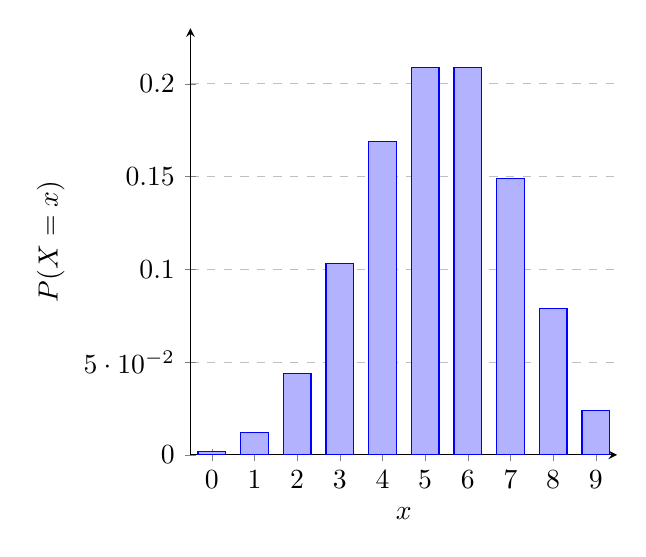
\begin{tikzpicture}
    \begin{axis}[
        ybar,
        bar width=10pt,
        width=7cm,
        height=7cm,
        ymin=0,
        ymax=0.23,
        xmin=-0.5,
        xmax=9.5,
        xtick={0,1,...,9},
        xlabel={$x$},
        ylabel={$P(X=x)$},
        axis lines=left,
        ymajorgrids,
        grid style={dashed},
    ]
        \addplot coordinates {
            (0,0.002)
            (1,0.012)
            (2,0.044)
            (3,0.103)
            (4,0.169)
            (5,0.209)
            (6,0.209)
            (7,0.149)
            (8,0.079)
            (9,0.024)
        };
    \end{axis}
\end{tikzpicture}
\end{center}

\begin{enumerate}
\item Quelle est la valeur la plus probable prise par (X) ?

\item Calculer approximativement \(P(X\leq3)\) à partir de la distribution.

\item Calculer approximativement \(P(X\geq6)\).

\item Que peut-on dire de la répartition des valeurs de \(X\) autour de sa valeur moyenne ?

\item Sans effectuer de calcul détaillé, expliquer pourquoi cette distribution permet de constater que certaines valeurs de \(X\) sont beaucoup plus probables que d'autres.

\end{enumerate}
\end{exo}


\section{Loi uniforme}


\begin{exo}[][appro]

Dans un laboratoire, un test est réalisé sur \(100\) échantillons.
On estime que la probabilité qu'un échantillon donne un résultat positif est de \(0,4\).
On suppose que les résultats des différents échantillons sont indépendants.

On note \(X\) le nombre de résultats positifs obtenus parmi les \(100\) échantillons.

\begin{enumerate}
    \item Justifier que \(X\) suit une loi binomiale et préciser ses paramètres.
    \item 
    \item À l'aide de l'histogramme ci-dessous, déterminer l'espérance de \(X\).
    
    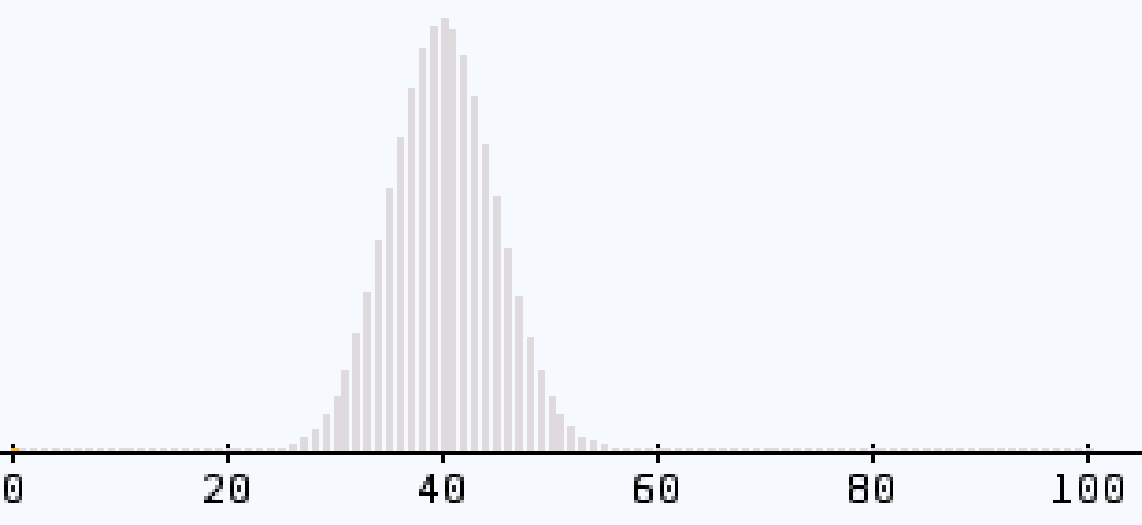
\includegraphics[width=7cm]{histo.png}
    \item Pour simplifier, on choisi de représenter la dostribution par une \textbf{courbe en cloche}.
    
    \begin{center}
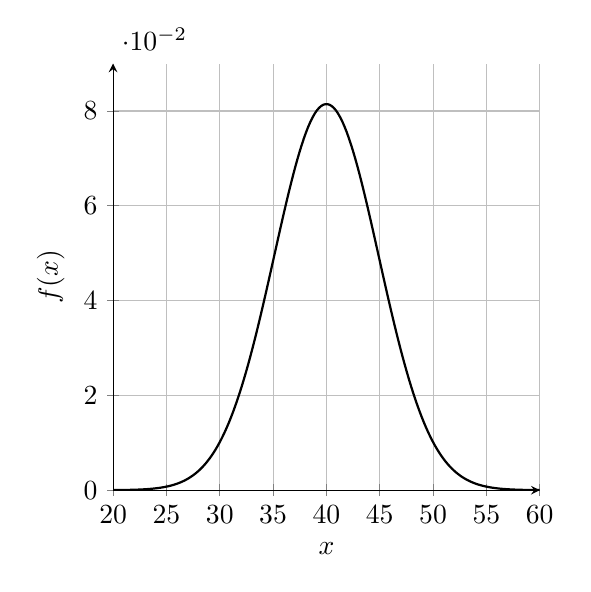
\begin{tikzpicture}
    \begin{axis}[
        width=7cm,
        height=7cm,
        xmin=20,
        xmax=60,
        ymin=0,
        ymax=0.09,
        axis lines=left,
        xlabel={$x$},
        ylabel={$f(x)$},
        xtick={20,25,...,60},
        ytick={0,0.02,0.04,0.06,0.08},
        grid=major,
    ]
        \addplot[
            domain=20:60,
            samples=200,
            thick
        ]
        {1/sqrt(48*pi)*exp(-(x-40)^2/48)};
    \end{axis}
\end{tikzpicture}
\end{center}

Comment pourrait-on calculer la probabilité d'avoir au moins \(45\) résultats positifs à partir de cette courbe ?
\end{enumerate}
\end{exo}

\prof{
Pour la question 3, remarquer que l'histogramme est symétrique.

    On peut poser des questions à l'oral ensuite, par exemple \(P(X\geq 40)\), comparer des probas, etc.

    Passer  au cours ensuite
}

\begin{exo}
Soit $X$ une variable aléatoire suivant la loi $\mathcal{N}(7,5;3)$. On note $f$ la densité de probabilité de cette loi et on l'a représenté ci-dessous :

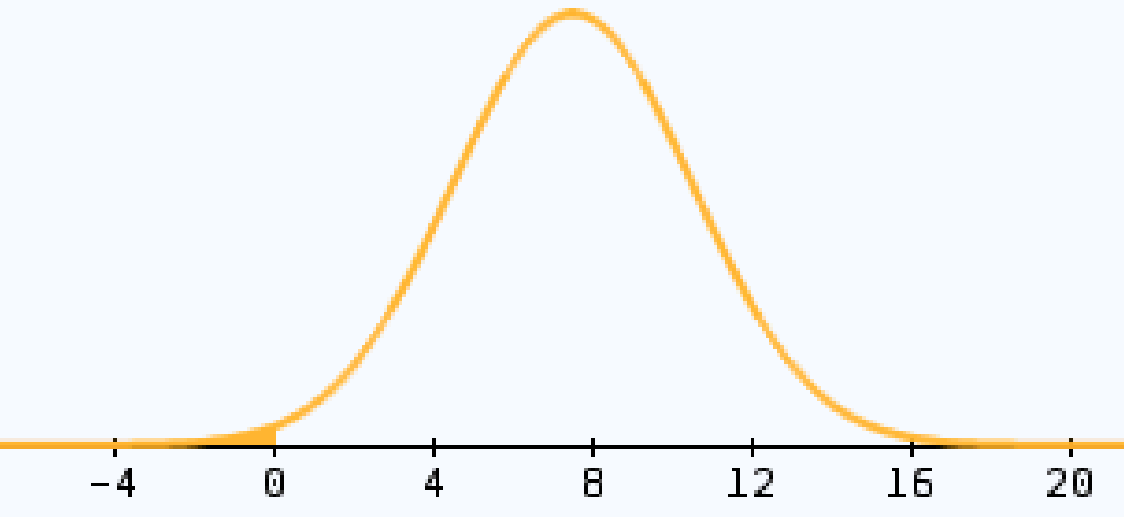
\includegraphics[width=0.3\textwidth]{fig/fig4.png}

\begin{enumerate}
\item Hachurer sur cette représentation les régions dont l'aire correspond à \begin{tasks}(2)
\task $P(X\leq 4)$
\task $P(8\leq X \leq 12)$
\end{tasks}
\item À l'aide de la calculatrice, calculer cette probabilité.
\end{enumerate}
\end{exo}

\begin{exo}
Relier les lois normales ci-dessous à leur fonction densité :\\
Lois :
\begin{tasks}(2)
\task $X\sim \mathcal{N}(30;5)$
\task $Y\sim \mathcal{N}(5;30)$
\task $Z\sim \mathcal{N}(5;5)$
\task $T\sim \mathcal{N}(30;30)$
\end{tasks}

Fonctions densité :
\begin{tasks}(2)
\task 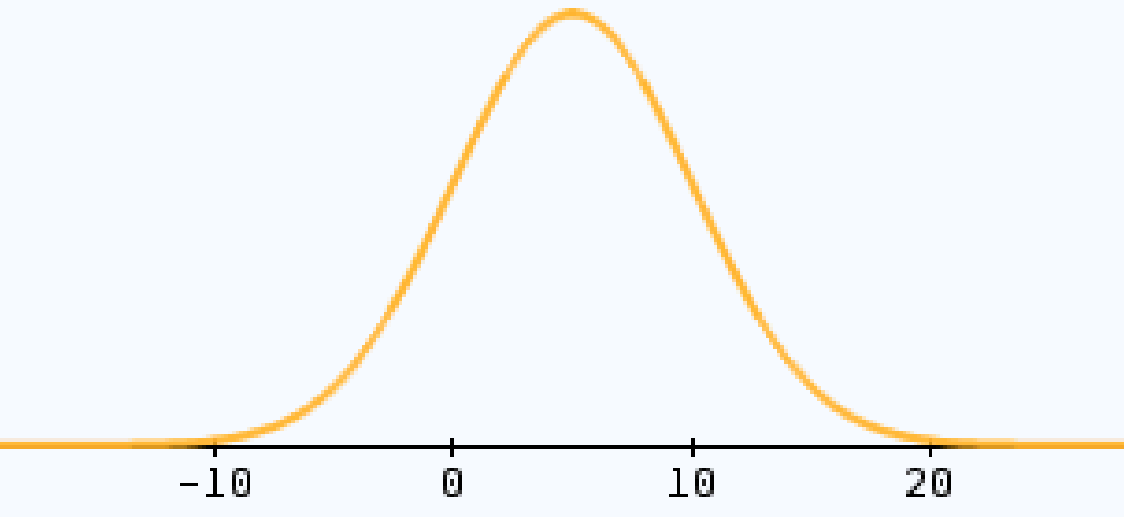
\includegraphics[width=0.2\textwidth]{fig/fig5.png}
\task 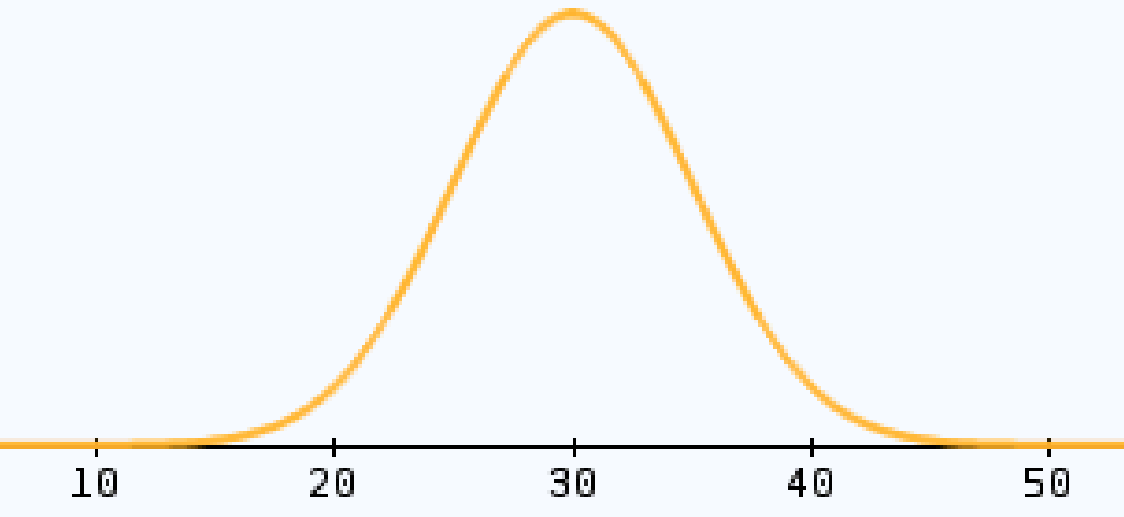
\includegraphics[width=0.2\textwidth]{fig/fig6.png}
\task 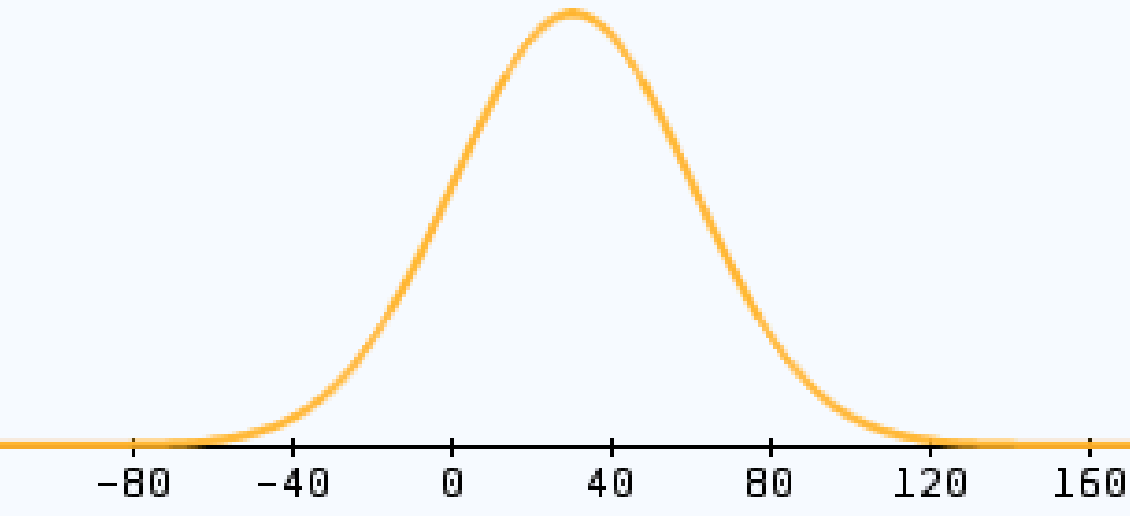
\includegraphics[width=0.2\textwidth]{fig/fig7.png}
\task 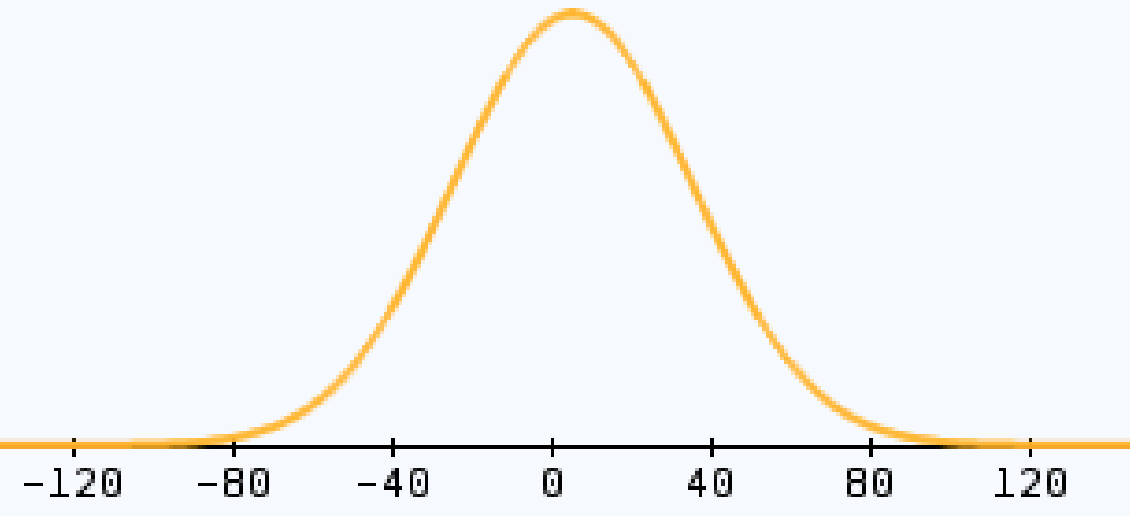
\includegraphics[width=0.2\textwidth]{fig/fig8.png}
\end{tasks}
\end{exo}



\begin{exo}[][]
    Dans une population donnée, la concentration (en mg/L) d'une substance dans le sang est modélisée par une variable aléatoire \(X\) suivant une loi normale de moyenne \(\mu = 100\) et d'écart-type \(\sigma = 12\).
    \begin{enumerate}
        \item Rappeler à quoi correspondent \(\mu\) et \(\sigma\).
        \item Calculer \(P(88\geq X\geq 112)\)
        \item Quelle est la probabilité qu'un individu ait une concentration supérieure à 124 mg/L ?
        \item Autour de quelles valeurs doit-être située la concentration pour que 95\% des individus aient une concentration comprise entre ces deux valeurs ?
        \item Autour de quelles valeurs doit-être située la concentration pour que 99,7\% des individus aient une concentration comprise entre ces deux valeurs ?
    \end{enumerate}
\end{exo}


\begin{exo}[][ccf]

\textbf{Les résultats seront arrondis au millième.}

Une entreprise pharmaceutique produit des flacons contenant une solution injectable. Chaque flacon est soumis à différents contrôles avant sa commercialisation.

\subsection*{Partie A -- Contrôle du volume}

On note \(X\) la variable aléatoire qui, à un flacon prélevé au hasard dans la production, associe son volume de solution, exprimé en mL.

L'étude statistique de la production permet de modéliser (X) par une loi normale de moyenne
\[
\mu=10
\]
et d'écart type
\[
\sigma=0,15.
\]

Un flacon est considéré comme conforme pour son volume si celui-ci appartient à l'intervalle
\[
[9,7,;,10,3].
\]

\begin{enumerate}
\item Calculer la probabilité qu'un flacon prélevé au hasard soit conforme pour son volume.

```
\item Calculer la probabilité qu'un flacon ait un volume inférieur ou égal à \(9,8\) mL.

\item Le responsable qualité souhaite que la proportion de flacons dont le volume est compris entre \(9,8\) mL et \(10,2\) mL soit supérieure à \(80\,\%\).

Cette exigence est-elle satisfaite ? Justifier.

\item Déterminer, à \(10^{-2}\) près, le nombre \(a>0\) tel que
\[
P(10-a\leq X\leq10+a)=0,95.
\]
Interpréter le résultat dans le contexte de l'entreprise.
```

\end{enumerate}

\subsection*{Partie B -- Contrôle d'un lot de flacons}

On s'intéresse maintenant à la conformité globale des flacons.

On estime que \(4,\%\) des flacons produits présentent au moins une non-conformité.

On prélève au hasard \(50\) flacons dans la production. La production étant suffisamment importante, on assimile ce prélèvement à \(50\) tirages indépendants.

On note \(Y\) la variable aléatoire qui compte le nombre de flacons non conformes parmi les \(50\) flacons prélevés.

\begin{enumerate}
\item Justifier que \(Y\) suit une loi binomiale dont on précisera les paramètres.

\item Calculer la probabilité que le prélèvement contienne exactement deux flacons non conformes.

\item Calculer la probabilité que le prélèvement contienne au plus trois flacons non conformes.

\item Le responsable qualité considère qu'un lot est acceptable si le prélèvement contient au maximum trois flacons non conformes.

Calculer la probabilité qu'un lot soit déclaré acceptable selon cette procédure.

\item Déterminer l'espérance et l'écart type de \(Y\). Interpréter ces deux résultats dans le contexte.


\end{enumerate}

\end{exo}
\end{multicols}


\end{document}
